\begin{frame}{Hierarchical Encondings}
  Hierarchical encodings are derived from \alert{hierarchical trees}.

  \metroset{block=fill}
  \begin{block}{Example}
    \begin{align*}
      \mathcal{C} &= [
        &\texttt{lemon} &,  &\texttt{pear} &,  &\texttt{apple} &,
        &\texttt{dog} &, &\texttt{cat} &, &\texttt{car} &\
      ]
    \end{align*}
    \tikzfig{figures/02/hierarchical_tree}
  \end{block}

  \note[item]{Una gererchia tra le classi è un'informazione che possiamo
  sfruttare per costruire una funzione di encoding che tenga conto delle
  relazioni tra queste.}
  \note[item]{Un modo di rappresentare una gerachia è con una struttura ad
  albero.}
  \note[item]{Limone, pera e mela sono frutti, cane e gatto animali mentre l'auto è
  un veicolo. Frutti e animali sono presenti in natura, i veicoli sono
  oggetti artificiali.}
  \note[item]{Questo è un esempio di gerarchia dalla quale possiamo
  derivare un embedding gerarchico.}
\end{frame}

\begin{frame}{Hierarchical Encondings}
  \begin{columns}
    \column{0.7\textwidth}
    \only<1>{\tikzfig{figures/02/lca}}
    \only<2>{\tikzfig{figures/02/similarity}}
    \only<3>{\tikzfig{figures/02/probability}}
    \only<4>{\tikzfig{figures/02/probability_apple}}

    \column{0.3\textwidth}
    \begin{enumerate}[<+- | alert@+>]
      \item distance
      \item similarity
      \item probability
    \end{enumerate}
  \end{columns}

  \note[item]{Iniziamo costruendo una matrice di distanza tra le classi per
  esempio usando l'altezza dell'ultimo antenato comune. Ogni classe ha distanza
  0 da se stessa. I frutti hanno distanza 1 tra loro, 2 con gli animali e 3,
  distanza massima con i veicoli.}
  \note[item]{Dalla distanza construiamo una matrice di similarità. 1 -
  distanza normalizzata. Le classi avranno similarità 1 con se stesse e 0 con
  quelle con cui non hanno niente in comune.}
  \note[item]{Infine, otteniamo una probability mass function sulle classi
  applicando la softmax lungo le righe. E ora ogni righa corrisponde
  all'encoding di una classe.}
  \note[item]{NEXT}
  \note[item]{Consideriamo l'encoding per la classe "mela".}
\end{frame}

\begin{frame}{Hierarchical Encondings}
  \only<1>{
    \centering
    similarity $\longrightarrow$ probability
    \vspace{-0.0cm}
    %% Creator: Matplotlib, PGF backend
%%
%% To include the figure in your LaTeX document, write
%%   \input{<filename>.pgf}
%%
%% Make sure the required packages are loaded in your preamble
%%   \usepackage{pgf}
%%
%% Also ensure that all the required font packages are loaded; for instance,
%% the lmodern package is sometimes necessary when using math font.
%%   \usepackage{lmodern}
%%
%% Figures using additional raster images can only be included by \input if
%% they are in the same directory as the main LaTeX file. For loading figures
%% from other directories you can use the `import` package
%%   \usepackage{import}
%%
%% and then include the figures with
%%   \import{<path to file>}{<filename>.pgf}
%%
%% Matplotlib used the following preamble
%%   
%%   \usepackage{fontspec}
%%   \setmainfont{DejaVuSerif.ttf}[Path=\detokenize{/Users/simo/.local/share/virtualenvs/master-thesis-code/lib/python3.10/site-packages/matplotlib/mpl-data/fonts/ttf/}]
%%   \setsansfont{DejaVuSans.ttf}[Path=\detokenize{/Users/simo/.local/share/virtualenvs/master-thesis-code/lib/python3.10/site-packages/matplotlib/mpl-data/fonts/ttf/}]
%%   \setmonofont{DejaVuSansMono.ttf}[Path=\detokenize{/Users/simo/.local/share/virtualenvs/master-thesis-code/lib/python3.10/site-packages/matplotlib/mpl-data/fonts/ttf/}]
%%   \makeatletter\@ifpackageloaded{underscore}{}{\usepackage[strings]{underscore}}\makeatother
%%
\begingroup%
\makeatletter%
\begin{pgfpicture}%
\pgfpathrectangle{\pgfpointorigin}{\pgfqpoint{4.251970in}{2.400000in}}%
\pgfusepath{use as bounding box, clip}%
\begin{pgfscope}%
\pgfsetbuttcap%
\pgfsetmiterjoin%
\definecolor{currentfill}{rgb}{0.980392,0.980392,0.980392}%
\pgfsetfillcolor{currentfill}%
\pgfsetlinewidth{0.000000pt}%
\definecolor{currentstroke}{rgb}{1.000000,1.000000,1.000000}%
\pgfsetstrokecolor{currentstroke}%
\pgfsetdash{}{0pt}%
\pgfpathmoveto{\pgfqpoint{0.000000in}{0.000000in}}%
\pgfpathlineto{\pgfqpoint{4.251970in}{0.000000in}}%
\pgfpathlineto{\pgfqpoint{4.251970in}{2.400000in}}%
\pgfpathlineto{\pgfqpoint{0.000000in}{2.400000in}}%
\pgfpathlineto{\pgfqpoint{0.000000in}{0.000000in}}%
\pgfpathclose%
\pgfusepath{fill}%
\end{pgfscope}%
\begin{pgfscope}%
\pgfsetbuttcap%
\pgfsetmiterjoin%
\definecolor{currentfill}{rgb}{0.917647,0.917647,0.949020}%
\pgfsetfillcolor{currentfill}%
\pgfsetlinewidth{0.000000pt}%
\definecolor{currentstroke}{rgb}{0.000000,0.000000,0.000000}%
\pgfsetstrokecolor{currentstroke}%
\pgfsetstrokeopacity{0.000000}%
\pgfsetdash{}{0pt}%
\pgfpathmoveto{\pgfqpoint{0.439176in}{0.313488in}}%
\pgfpathlineto{\pgfqpoint{4.101970in}{0.313488in}}%
\pgfpathlineto{\pgfqpoint{4.101970in}{2.250000in}}%
\pgfpathlineto{\pgfqpoint{0.439176in}{2.250000in}}%
\pgfpathlineto{\pgfqpoint{0.439176in}{0.313488in}}%
\pgfpathclose%
\pgfusepath{fill}%
\end{pgfscope}%
\begin{pgfscope}%
\definecolor{textcolor}{rgb}{0.137255,0.215686,0.231373}%
\pgfsetstrokecolor{textcolor}%
\pgfsetfillcolor{textcolor}%
\pgftext[x=0.835309in,y=0.174599in,,base]{\color{textcolor}\sffamily\fontsize{8.000000}{9.600000}\selectfont \texttt{lemon}}%
\end{pgfscope}%
\begin{pgfscope}%
\definecolor{textcolor}{rgb}{0.137255,0.215686,0.231373}%
\pgfsetstrokecolor{textcolor}%
\pgfsetfillcolor{textcolor}%
\pgftext[x=1.409415in,y=0.174599in,,base]{\color{textcolor}\sffamily\fontsize{8.000000}{9.600000}\selectfont \texttt{pear}}%
\end{pgfscope}%
\begin{pgfscope}%
\definecolor{textcolor}{rgb}{0.137255,0.215686,0.231373}%
\pgfsetstrokecolor{textcolor}%
\pgfsetfillcolor{textcolor}%
\pgftext[x=1.983520in,y=0.174599in,,base]{\color{textcolor}\sffamily\fontsize{8.000000}{9.600000}\selectfont \texttt{apple}}%
\end{pgfscope}%
\begin{pgfscope}%
\definecolor{textcolor}{rgb}{0.137255,0.215686,0.231373}%
\pgfsetstrokecolor{textcolor}%
\pgfsetfillcolor{textcolor}%
\pgftext[x=2.557626in,y=0.174599in,,base]{\color{textcolor}\sffamily\fontsize{8.000000}{9.600000}\selectfont \texttt{dog}}%
\end{pgfscope}%
\begin{pgfscope}%
\definecolor{textcolor}{rgb}{0.137255,0.215686,0.231373}%
\pgfsetstrokecolor{textcolor}%
\pgfsetfillcolor{textcolor}%
\pgftext[x=3.131732in,y=0.174599in,,base]{\color{textcolor}\sffamily\fontsize{8.000000}{9.600000}\selectfont \texttt{cat}}%
\end{pgfscope}%
\begin{pgfscope}%
\definecolor{textcolor}{rgb}{0.137255,0.215686,0.231373}%
\pgfsetstrokecolor{textcolor}%
\pgfsetfillcolor{textcolor}%
\pgftext[x=3.705837in,y=0.174599in,,base]{\color{textcolor}\sffamily\fontsize{8.000000}{9.600000}\selectfont \texttt{car}}%
\end{pgfscope}%
\begin{pgfscope}%
\definecolor{textcolor}{rgb}{0.137255,0.215686,0.231373}%
\pgfsetstrokecolor{textcolor}%
\pgfsetfillcolor{textcolor}%
\pgftext[x=0.149436in, y=0.271279in, left, base]{\color{textcolor}\sffamily\fontsize{8.000000}{9.600000}\selectfont \(\displaystyle {0.0}\)}%
\end{pgfscope}%
\begin{pgfscope}%
\definecolor{textcolor}{rgb}{0.137255,0.215686,0.231373}%
\pgfsetstrokecolor{textcolor}%
\pgfsetfillcolor{textcolor}%
\pgftext[x=0.149436in, y=0.623372in, left, base]{\color{textcolor}\sffamily\fontsize{8.000000}{9.600000}\selectfont \(\displaystyle {0.2}\)}%
\end{pgfscope}%
\begin{pgfscope}%
\definecolor{textcolor}{rgb}{0.137255,0.215686,0.231373}%
\pgfsetstrokecolor{textcolor}%
\pgfsetfillcolor{textcolor}%
\pgftext[x=0.149436in, y=0.975465in, left, base]{\color{textcolor}\sffamily\fontsize{8.000000}{9.600000}\selectfont \(\displaystyle {0.4}\)}%
\end{pgfscope}%
\begin{pgfscope}%
\definecolor{textcolor}{rgb}{0.137255,0.215686,0.231373}%
\pgfsetstrokecolor{textcolor}%
\pgfsetfillcolor{textcolor}%
\pgftext[x=0.149436in, y=1.327558in, left, base]{\color{textcolor}\sffamily\fontsize{8.000000}{9.600000}\selectfont \(\displaystyle {0.6}\)}%
\end{pgfscope}%
\begin{pgfscope}%
\definecolor{textcolor}{rgb}{0.137255,0.215686,0.231373}%
\pgfsetstrokecolor{textcolor}%
\pgfsetfillcolor{textcolor}%
\pgftext[x=0.149436in, y=1.679651in, left, base]{\color{textcolor}\sffamily\fontsize{8.000000}{9.600000}\selectfont \(\displaystyle {0.8}\)}%
\end{pgfscope}%
\begin{pgfscope}%
\definecolor{textcolor}{rgb}{0.137255,0.215686,0.231373}%
\pgfsetstrokecolor{textcolor}%
\pgfsetfillcolor{textcolor}%
\pgftext[x=0.149436in, y=2.031744in, left, base]{\color{textcolor}\sffamily\fontsize{8.000000}{9.600000}\selectfont \(\displaystyle {1.0}\)}%
\end{pgfscope}%
\begin{pgfscope}%
\pgfpathrectangle{\pgfqpoint{0.439176in}{0.313488in}}{\pgfqpoint{3.662794in}{1.936512in}}%
\pgfusepath{clip}%
\pgfsetbuttcap%
\pgfsetmiterjoin%
\definecolor{currentfill}{rgb}{0.623529,0.780392,1.000000}%
\pgfsetfillcolor{currentfill}%
\pgfsetlinewidth{1.505625pt}%
\definecolor{currentstroke}{rgb}{0.298039,0.447059,0.690196}%
\pgfsetstrokecolor{currentstroke}%
\pgfsetdash{}{0pt}%
\pgfpathmoveto{\pgfqpoint{0.605667in}{0.313488in}}%
\pgfpathlineto{\pgfqpoint{1.064951in}{0.313488in}}%
\pgfpathlineto{\pgfqpoint{1.064951in}{0.643034in}}%
\pgfpathlineto{\pgfqpoint{0.605667in}{0.643034in}}%
\pgfpathlineto{\pgfqpoint{0.605667in}{0.313488in}}%
\pgfpathclose%
\pgfusepath{stroke,fill}%
\end{pgfscope}%
\begin{pgfscope}%
\pgfpathrectangle{\pgfqpoint{0.439176in}{0.313488in}}{\pgfqpoint{3.662794in}{1.936512in}}%
\pgfusepath{clip}%
\pgfsetbuttcap%
\pgfsetmiterjoin%
\definecolor{currentfill}{rgb}{0.623529,0.780392,1.000000}%
\pgfsetfillcolor{currentfill}%
\pgfsetlinewidth{1.505625pt}%
\definecolor{currentstroke}{rgb}{0.298039,0.447059,0.690196}%
\pgfsetstrokecolor{currentstroke}%
\pgfsetdash{}{0pt}%
\pgfpathmoveto{\pgfqpoint{1.179772in}{0.313488in}}%
\pgfpathlineto{\pgfqpoint{1.639057in}{0.313488in}}%
\pgfpathlineto{\pgfqpoint{1.639057in}{0.643034in}}%
\pgfpathlineto{\pgfqpoint{1.179772in}{0.643034in}}%
\pgfpathlineto{\pgfqpoint{1.179772in}{0.313488in}}%
\pgfpathclose%
\pgfusepath{stroke,fill}%
\end{pgfscope}%
\begin{pgfscope}%
\pgfpathrectangle{\pgfqpoint{0.439176in}{0.313488in}}{\pgfqpoint{3.662794in}{1.936512in}}%
\pgfusepath{clip}%
\pgfsetbuttcap%
\pgfsetmiterjoin%
\definecolor{currentfill}{rgb}{0.623529,0.780392,1.000000}%
\pgfsetfillcolor{currentfill}%
\pgfsetlinewidth{1.505625pt}%
\definecolor{currentstroke}{rgb}{0.298039,0.447059,0.690196}%
\pgfsetstrokecolor{currentstroke}%
\pgfsetdash{}{0pt}%
\pgfpathmoveto{\pgfqpoint{1.753878in}{0.313488in}}%
\pgfpathlineto{\pgfqpoint{2.213163in}{0.313488in}}%
\pgfpathlineto{\pgfqpoint{2.213163in}{0.773407in}}%
\pgfpathlineto{\pgfqpoint{1.753878in}{0.773407in}}%
\pgfpathlineto{\pgfqpoint{1.753878in}{0.313488in}}%
\pgfpathclose%
\pgfusepath{stroke,fill}%
\end{pgfscope}%
\begin{pgfscope}%
\pgfpathrectangle{\pgfqpoint{0.439176in}{0.313488in}}{\pgfqpoint{3.662794in}{1.936512in}}%
\pgfusepath{clip}%
\pgfsetbuttcap%
\pgfsetmiterjoin%
\definecolor{currentfill}{rgb}{0.623529,0.780392,1.000000}%
\pgfsetfillcolor{currentfill}%
\pgfsetlinewidth{1.505625pt}%
\definecolor{currentstroke}{rgb}{0.298039,0.447059,0.690196}%
\pgfsetstrokecolor{currentstroke}%
\pgfsetdash{}{0pt}%
\pgfpathmoveto{\pgfqpoint{2.327984in}{0.313488in}}%
\pgfpathlineto{\pgfqpoint{2.787268in}{0.313488in}}%
\pgfpathlineto{\pgfqpoint{2.787268in}{0.549618in}}%
\pgfpathlineto{\pgfqpoint{2.327984in}{0.549618in}}%
\pgfpathlineto{\pgfqpoint{2.327984in}{0.313488in}}%
\pgfpathclose%
\pgfusepath{stroke,fill}%
\end{pgfscope}%
\begin{pgfscope}%
\pgfpathrectangle{\pgfqpoint{0.439176in}{0.313488in}}{\pgfqpoint{3.662794in}{1.936512in}}%
\pgfusepath{clip}%
\pgfsetbuttcap%
\pgfsetmiterjoin%
\definecolor{currentfill}{rgb}{0.623529,0.780392,1.000000}%
\pgfsetfillcolor{currentfill}%
\pgfsetlinewidth{1.505625pt}%
\definecolor{currentstroke}{rgb}{0.298039,0.447059,0.690196}%
\pgfsetstrokecolor{currentstroke}%
\pgfsetdash{}{0pt}%
\pgfpathmoveto{\pgfqpoint{2.902089in}{0.313488in}}%
\pgfpathlineto{\pgfqpoint{3.361374in}{0.313488in}}%
\pgfpathlineto{\pgfqpoint{3.361374in}{0.549618in}}%
\pgfpathlineto{\pgfqpoint{2.902089in}{0.549618in}}%
\pgfpathlineto{\pgfqpoint{2.902089in}{0.313488in}}%
\pgfpathclose%
\pgfusepath{stroke,fill}%
\end{pgfscope}%
\begin{pgfscope}%
\pgfpathrectangle{\pgfqpoint{0.439176in}{0.313488in}}{\pgfqpoint{3.662794in}{1.936512in}}%
\pgfusepath{clip}%
\pgfsetbuttcap%
\pgfsetmiterjoin%
\definecolor{currentfill}{rgb}{0.623529,0.780392,1.000000}%
\pgfsetfillcolor{currentfill}%
\pgfsetlinewidth{1.505625pt}%
\definecolor{currentstroke}{rgb}{0.298039,0.447059,0.690196}%
\pgfsetstrokecolor{currentstroke}%
\pgfsetdash{}{0pt}%
\pgfpathmoveto{\pgfqpoint{3.476195in}{0.313488in}}%
\pgfpathlineto{\pgfqpoint{3.935479in}{0.313488in}}%
\pgfpathlineto{\pgfqpoint{3.935479in}{0.482683in}}%
\pgfpathlineto{\pgfqpoint{3.476195in}{0.482683in}}%
\pgfpathlineto{\pgfqpoint{3.476195in}{0.313488in}}%
\pgfpathclose%
\pgfusepath{stroke,fill}%
\end{pgfscope}%
\begin{pgfscope}%
\pgfsetrectcap%
\pgfsetmiterjoin%
\pgfsetlinewidth{1.003750pt}%
\definecolor{currentstroke}{rgb}{0.917647,0.917647,0.949020}%
\pgfsetstrokecolor{currentstroke}%
\pgfsetdash{}{0pt}%
\pgfpathmoveto{\pgfqpoint{0.439176in}{0.313488in}}%
\pgfpathlineto{\pgfqpoint{0.439176in}{2.250000in}}%
\pgfusepath{stroke}%
\end{pgfscope}%
\begin{pgfscope}%
\pgfsetrectcap%
\pgfsetmiterjoin%
\pgfsetlinewidth{1.003750pt}%
\definecolor{currentstroke}{rgb}{0.917647,0.917647,0.949020}%
\pgfsetstrokecolor{currentstroke}%
\pgfsetdash{}{0pt}%
\pgfpathmoveto{\pgfqpoint{4.101970in}{0.313488in}}%
\pgfpathlineto{\pgfqpoint{4.101970in}{2.250000in}}%
\pgfusepath{stroke}%
\end{pgfscope}%
\begin{pgfscope}%
\pgfsetrectcap%
\pgfsetmiterjoin%
\pgfsetlinewidth{1.003750pt}%
\definecolor{currentstroke}{rgb}{0.917647,0.917647,0.949020}%
\pgfsetstrokecolor{currentstroke}%
\pgfsetdash{}{0pt}%
\pgfpathmoveto{\pgfqpoint{0.439176in}{0.313488in}}%
\pgfpathlineto{\pgfqpoint{4.101970in}{0.313488in}}%
\pgfusepath{stroke}%
\end{pgfscope}%
\begin{pgfscope}%
\pgfsetrectcap%
\pgfsetmiterjoin%
\pgfsetlinewidth{1.003750pt}%
\definecolor{currentstroke}{rgb}{0.917647,0.917647,0.949020}%
\pgfsetstrokecolor{currentstroke}%
\pgfsetdash{}{0pt}%
\pgfpathmoveto{\pgfqpoint{0.439176in}{2.250000in}}%
\pgfpathlineto{\pgfqpoint{4.101970in}{2.250000in}}%
\pgfusepath{stroke}%
\end{pgfscope}%
\begin{pgfscope}%
\pgfsetbuttcap%
\pgfsetmiterjoin%
\definecolor{currentfill}{rgb}{0.623529,0.780392,1.000000}%
\pgfsetfillcolor{currentfill}%
\pgfsetlinewidth{1.505625pt}%
\definecolor{currentstroke}{rgb}{0.298039,0.447059,0.690196}%
\pgfsetstrokecolor{currentstroke}%
\pgfsetdash{}{0pt}%
\pgfpathmoveto{\pgfqpoint{2.932915in}{2.018731in}}%
\pgfpathlineto{\pgfqpoint{3.210693in}{2.018731in}}%
\pgfpathlineto{\pgfqpoint{3.210693in}{2.115953in}}%
\pgfpathlineto{\pgfqpoint{2.932915in}{2.115953in}}%
\pgfpathlineto{\pgfqpoint{2.932915in}{2.018731in}}%
\pgfpathclose%
\pgfusepath{stroke,fill}%
\end{pgfscope}%
\begin{pgfscope}%
\definecolor{textcolor}{rgb}{0.137255,0.215686,0.231373}%
\pgfsetstrokecolor{textcolor}%
\pgfsetfillcolor{textcolor}%
\pgftext[x=3.321804in,y=2.018731in,left,base]{\color{textcolor}\sffamily\fontsize{10.000000}{12.000000}\selectfont \(\displaystyle \phi\,\left(\texttt{apple}\right)\)}%
\end{pgfscope}%
\end{pgfpicture}%
\makeatother%
\endgroup%

  }
  \only<2>{
    \centering
    similarity + hyperparam $\longrightarrow$ probability
    \vspace{-0.0cm}
    %% Creator: Matplotlib, PGF backend
%%
%% To include the figure in your LaTeX document, write
%%   \input{<filename>.pgf}
%%
%% Make sure the required packages are loaded in your preamble
%%   \usepackage{pgf}
%%
%% Also ensure that all the required font packages are loaded; for instance,
%% the lmodern package is sometimes necessary when using math font.
%%   \usepackage{lmodern}
%%
%% Figures using additional raster images can only be included by \input if
%% they are in the same directory as the main LaTeX file. For loading figures
%% from other directories you can use the `import` package
%%   \usepackage{import}
%%
%% and then include the figures with
%%   \import{<path to file>}{<filename>.pgf}
%%
%% Matplotlib used the following preamble
%%   
%%   \usepackage{fontspec}
%%   \setmainfont{DejaVuSerif.ttf}[Path=\detokenize{/Users/simo/.local/share/virtualenvs/master-thesis-code/lib/python3.10/site-packages/matplotlib/mpl-data/fonts/ttf/}]
%%   \setsansfont{DejaVuSans.ttf}[Path=\detokenize{/Users/simo/.local/share/virtualenvs/master-thesis-code/lib/python3.10/site-packages/matplotlib/mpl-data/fonts/ttf/}]
%%   \setmonofont{DejaVuSansMono.ttf}[Path=\detokenize{/Users/simo/.local/share/virtualenvs/master-thesis-code/lib/python3.10/site-packages/matplotlib/mpl-data/fonts/ttf/}]
%%   \makeatletter\@ifpackageloaded{underscore}{}{\usepackage[strings]{underscore}}\makeatother
%%
\begingroup%
\makeatletter%
\begin{pgfpicture}%
\pgfpathrectangle{\pgfpointorigin}{\pgfqpoint{4.251970in}{2.400000in}}%
\pgfusepath{use as bounding box, clip}%
\begin{pgfscope}%
\pgfsetbuttcap%
\pgfsetmiterjoin%
\definecolor{currentfill}{rgb}{0.980392,0.980392,0.980392}%
\pgfsetfillcolor{currentfill}%
\pgfsetlinewidth{0.000000pt}%
\definecolor{currentstroke}{rgb}{1.000000,1.000000,1.000000}%
\pgfsetstrokecolor{currentstroke}%
\pgfsetdash{}{0pt}%
\pgfpathmoveto{\pgfqpoint{0.000000in}{0.000000in}}%
\pgfpathlineto{\pgfqpoint{4.251970in}{0.000000in}}%
\pgfpathlineto{\pgfqpoint{4.251970in}{2.400000in}}%
\pgfpathlineto{\pgfqpoint{0.000000in}{2.400000in}}%
\pgfpathlineto{\pgfqpoint{0.000000in}{0.000000in}}%
\pgfpathclose%
\pgfusepath{fill}%
\end{pgfscope}%
\begin{pgfscope}%
\pgfsetbuttcap%
\pgfsetmiterjoin%
\definecolor{currentfill}{rgb}{0.917647,0.917647,0.949020}%
\pgfsetfillcolor{currentfill}%
\pgfsetlinewidth{0.000000pt}%
\definecolor{currentstroke}{rgb}{0.000000,0.000000,0.000000}%
\pgfsetstrokecolor{currentstroke}%
\pgfsetstrokeopacity{0.000000}%
\pgfsetdash{}{0pt}%
\pgfpathmoveto{\pgfqpoint{0.439176in}{0.313488in}}%
\pgfpathlineto{\pgfqpoint{4.101970in}{0.313488in}}%
\pgfpathlineto{\pgfqpoint{4.101970in}{2.250000in}}%
\pgfpathlineto{\pgfqpoint{0.439176in}{2.250000in}}%
\pgfpathlineto{\pgfqpoint{0.439176in}{0.313488in}}%
\pgfpathclose%
\pgfusepath{fill}%
\end{pgfscope}%
\begin{pgfscope}%
\definecolor{textcolor}{rgb}{0.137255,0.215686,0.231373}%
\pgfsetstrokecolor{textcolor}%
\pgfsetfillcolor{textcolor}%
\pgftext[x=0.684948in,y=0.174599in,,base]{\color{textcolor}\sffamily\fontsize{8.000000}{9.600000}\selectfont \texttt{lemon}}%
\end{pgfscope}%
\begin{pgfscope}%
\definecolor{textcolor}{rgb}{0.137255,0.215686,0.231373}%
\pgfsetstrokecolor{textcolor}%
\pgfsetfillcolor{textcolor}%
\pgftext[x=1.319198in,y=0.174599in,,base]{\color{textcolor}\sffamily\fontsize{8.000000}{9.600000}\selectfont \texttt{pear}}%
\end{pgfscope}%
\begin{pgfscope}%
\definecolor{textcolor}{rgb}{0.137255,0.215686,0.231373}%
\pgfsetstrokecolor{textcolor}%
\pgfsetfillcolor{textcolor}%
\pgftext[x=1.953448in,y=0.174599in,,base]{\color{textcolor}\sffamily\fontsize{8.000000}{9.600000}\selectfont \texttt{apple}}%
\end{pgfscope}%
\begin{pgfscope}%
\definecolor{textcolor}{rgb}{0.137255,0.215686,0.231373}%
\pgfsetstrokecolor{textcolor}%
\pgfsetfillcolor{textcolor}%
\pgftext[x=2.587698in,y=0.174599in,,base]{\color{textcolor}\sffamily\fontsize{8.000000}{9.600000}\selectfont \texttt{dog}}%
\end{pgfscope}%
\begin{pgfscope}%
\definecolor{textcolor}{rgb}{0.137255,0.215686,0.231373}%
\pgfsetstrokecolor{textcolor}%
\pgfsetfillcolor{textcolor}%
\pgftext[x=3.221948in,y=0.174599in,,base]{\color{textcolor}\sffamily\fontsize{8.000000}{9.600000}\selectfont \texttt{cat}}%
\end{pgfscope}%
\begin{pgfscope}%
\definecolor{textcolor}{rgb}{0.137255,0.215686,0.231373}%
\pgfsetstrokecolor{textcolor}%
\pgfsetfillcolor{textcolor}%
\pgftext[x=3.856198in,y=0.174599in,,base]{\color{textcolor}\sffamily\fontsize{8.000000}{9.600000}\selectfont \texttt{car}}%
\end{pgfscope}%
\begin{pgfscope}%
\definecolor{textcolor}{rgb}{0.137255,0.215686,0.231373}%
\pgfsetstrokecolor{textcolor}%
\pgfsetfillcolor{textcolor}%
\pgftext[x=0.149436in, y=0.271279in, left, base]{\color{textcolor}\sffamily\fontsize{8.000000}{9.600000}\selectfont \(\displaystyle {0.0}\)}%
\end{pgfscope}%
\begin{pgfscope}%
\definecolor{textcolor}{rgb}{0.137255,0.215686,0.231373}%
\pgfsetstrokecolor{textcolor}%
\pgfsetfillcolor{textcolor}%
\pgftext[x=0.149436in, y=0.623372in, left, base]{\color{textcolor}\sffamily\fontsize{8.000000}{9.600000}\selectfont \(\displaystyle {0.2}\)}%
\end{pgfscope}%
\begin{pgfscope}%
\definecolor{textcolor}{rgb}{0.137255,0.215686,0.231373}%
\pgfsetstrokecolor{textcolor}%
\pgfsetfillcolor{textcolor}%
\pgftext[x=0.149436in, y=0.975465in, left, base]{\color{textcolor}\sffamily\fontsize{8.000000}{9.600000}\selectfont \(\displaystyle {0.4}\)}%
\end{pgfscope}%
\begin{pgfscope}%
\definecolor{textcolor}{rgb}{0.137255,0.215686,0.231373}%
\pgfsetstrokecolor{textcolor}%
\pgfsetfillcolor{textcolor}%
\pgftext[x=0.149436in, y=1.327558in, left, base]{\color{textcolor}\sffamily\fontsize{8.000000}{9.600000}\selectfont \(\displaystyle {0.6}\)}%
\end{pgfscope}%
\begin{pgfscope}%
\definecolor{textcolor}{rgb}{0.137255,0.215686,0.231373}%
\pgfsetstrokecolor{textcolor}%
\pgfsetfillcolor{textcolor}%
\pgftext[x=0.149436in, y=1.679651in, left, base]{\color{textcolor}\sffamily\fontsize{8.000000}{9.600000}\selectfont \(\displaystyle {0.8}\)}%
\end{pgfscope}%
\begin{pgfscope}%
\definecolor{textcolor}{rgb}{0.137255,0.215686,0.231373}%
\pgfsetstrokecolor{textcolor}%
\pgfsetfillcolor{textcolor}%
\pgftext[x=0.149436in, y=2.031744in, left, base]{\color{textcolor}\sffamily\fontsize{8.000000}{9.600000}\selectfont \(\displaystyle {1.0}\)}%
\end{pgfscope}%
\begin{pgfscope}%
\pgfpathrectangle{\pgfqpoint{0.439176in}{0.313488in}}{\pgfqpoint{3.662794in}{1.936512in}}%
\pgfusepath{clip}%
\pgfsetbuttcap%
\pgfsetmiterjoin%
\definecolor{currentfill}{rgb}{0.623529,0.780392,1.000000}%
\pgfsetfillcolor{currentfill}%
\pgfsetlinewidth{1.505625pt}%
\definecolor{currentstroke}{rgb}{0.298039,0.447059,0.690196}%
\pgfsetstrokecolor{currentstroke}%
\pgfsetdash{}{0pt}%
\pgfpathmoveto{\pgfqpoint{0.605667in}{0.313488in}}%
\pgfpathlineto{\pgfqpoint{0.764229in}{0.313488in}}%
\pgfpathlineto{\pgfqpoint{0.764229in}{0.588976in}}%
\pgfpathlineto{\pgfqpoint{0.605667in}{0.588976in}}%
\pgfpathlineto{\pgfqpoint{0.605667in}{0.313488in}}%
\pgfpathclose%
\pgfusepath{stroke,fill}%
\end{pgfscope}%
\begin{pgfscope}%
\pgfpathrectangle{\pgfqpoint{0.439176in}{0.313488in}}{\pgfqpoint{3.662794in}{1.936512in}}%
\pgfusepath{clip}%
\pgfsetbuttcap%
\pgfsetmiterjoin%
\definecolor{currentfill}{rgb}{0.623529,0.780392,1.000000}%
\pgfsetfillcolor{currentfill}%
\pgfsetlinewidth{1.505625pt}%
\definecolor{currentstroke}{rgb}{0.298039,0.447059,0.690196}%
\pgfsetstrokecolor{currentstroke}%
\pgfsetdash{}{0pt}%
\pgfpathmoveto{\pgfqpoint{1.239917in}{0.313488in}}%
\pgfpathlineto{\pgfqpoint{1.398479in}{0.313488in}}%
\pgfpathlineto{\pgfqpoint{1.398479in}{0.588976in}}%
\pgfpathlineto{\pgfqpoint{1.239917in}{0.588976in}}%
\pgfpathlineto{\pgfqpoint{1.239917in}{0.313488in}}%
\pgfpathclose%
\pgfusepath{stroke,fill}%
\end{pgfscope}%
\begin{pgfscope}%
\pgfpathrectangle{\pgfqpoint{0.439176in}{0.313488in}}{\pgfqpoint{3.662794in}{1.936512in}}%
\pgfusepath{clip}%
\pgfsetbuttcap%
\pgfsetmiterjoin%
\definecolor{currentfill}{rgb}{0.623529,0.780392,1.000000}%
\pgfsetfillcolor{currentfill}%
\pgfsetlinewidth{1.505625pt}%
\definecolor{currentstroke}{rgb}{0.298039,0.447059,0.690196}%
\pgfsetstrokecolor{currentstroke}%
\pgfsetdash{}{0pt}%
\pgfpathmoveto{\pgfqpoint{1.874167in}{0.313488in}}%
\pgfpathlineto{\pgfqpoint{2.032729in}{0.313488in}}%
\pgfpathlineto{\pgfqpoint{2.032729in}{1.358599in}}%
\pgfpathlineto{\pgfqpoint{1.874167in}{1.358599in}}%
\pgfpathlineto{\pgfqpoint{1.874167in}{0.313488in}}%
\pgfpathclose%
\pgfusepath{stroke,fill}%
\end{pgfscope}%
\begin{pgfscope}%
\pgfpathrectangle{\pgfqpoint{0.439176in}{0.313488in}}{\pgfqpoint{3.662794in}{1.936512in}}%
\pgfusepath{clip}%
\pgfsetbuttcap%
\pgfsetmiterjoin%
\definecolor{currentfill}{rgb}{0.623529,0.780392,1.000000}%
\pgfsetfillcolor{currentfill}%
\pgfsetlinewidth{1.505625pt}%
\definecolor{currentstroke}{rgb}{0.298039,0.447059,0.690196}%
\pgfsetstrokecolor{currentstroke}%
\pgfsetdash{}{0pt}%
\pgfpathmoveto{\pgfqpoint{2.508417in}{0.313488in}}%
\pgfpathlineto{\pgfqpoint{2.666979in}{0.313488in}}%
\pgfpathlineto{\pgfqpoint{2.666979in}{0.386106in}}%
\pgfpathlineto{\pgfqpoint{2.508417in}{0.386106in}}%
\pgfpathlineto{\pgfqpoint{2.508417in}{0.313488in}}%
\pgfpathclose%
\pgfusepath{stroke,fill}%
\end{pgfscope}%
\begin{pgfscope}%
\pgfpathrectangle{\pgfqpoint{0.439176in}{0.313488in}}{\pgfqpoint{3.662794in}{1.936512in}}%
\pgfusepath{clip}%
\pgfsetbuttcap%
\pgfsetmiterjoin%
\definecolor{currentfill}{rgb}{0.623529,0.780392,1.000000}%
\pgfsetfillcolor{currentfill}%
\pgfsetlinewidth{1.505625pt}%
\definecolor{currentstroke}{rgb}{0.298039,0.447059,0.690196}%
\pgfsetstrokecolor{currentstroke}%
\pgfsetdash{}{0pt}%
\pgfpathmoveto{\pgfqpoint{3.142667in}{0.313488in}}%
\pgfpathlineto{\pgfqpoint{3.301229in}{0.313488in}}%
\pgfpathlineto{\pgfqpoint{3.301229in}{0.386106in}}%
\pgfpathlineto{\pgfqpoint{3.142667in}{0.386106in}}%
\pgfpathlineto{\pgfqpoint{3.142667in}{0.313488in}}%
\pgfpathclose%
\pgfusepath{stroke,fill}%
\end{pgfscope}%
\begin{pgfscope}%
\pgfpathrectangle{\pgfqpoint{0.439176in}{0.313488in}}{\pgfqpoint{3.662794in}{1.936512in}}%
\pgfusepath{clip}%
\pgfsetbuttcap%
\pgfsetmiterjoin%
\definecolor{currentfill}{rgb}{0.623529,0.780392,1.000000}%
\pgfsetfillcolor{currentfill}%
\pgfsetlinewidth{1.505625pt}%
\definecolor{currentstroke}{rgb}{0.298039,0.447059,0.690196}%
\pgfsetstrokecolor{currentstroke}%
\pgfsetdash{}{0pt}%
\pgfpathmoveto{\pgfqpoint{3.776917in}{0.313488in}}%
\pgfpathlineto{\pgfqpoint{3.935479in}{0.313488in}}%
\pgfpathlineto{\pgfqpoint{3.935479in}{0.332630in}}%
\pgfpathlineto{\pgfqpoint{3.776917in}{0.332630in}}%
\pgfpathlineto{\pgfqpoint{3.776917in}{0.313488in}}%
\pgfpathclose%
\pgfusepath{stroke,fill}%
\end{pgfscope}%
\begin{pgfscope}%
\pgfsetrectcap%
\pgfsetmiterjoin%
\pgfsetlinewidth{1.003750pt}%
\definecolor{currentstroke}{rgb}{0.917647,0.917647,0.949020}%
\pgfsetstrokecolor{currentstroke}%
\pgfsetdash{}{0pt}%
\pgfpathmoveto{\pgfqpoint{0.439176in}{0.313488in}}%
\pgfpathlineto{\pgfqpoint{0.439176in}{2.250000in}}%
\pgfusepath{stroke}%
\end{pgfscope}%
\begin{pgfscope}%
\pgfsetrectcap%
\pgfsetmiterjoin%
\pgfsetlinewidth{1.003750pt}%
\definecolor{currentstroke}{rgb}{0.917647,0.917647,0.949020}%
\pgfsetstrokecolor{currentstroke}%
\pgfsetdash{}{0pt}%
\pgfpathmoveto{\pgfqpoint{4.101970in}{0.313488in}}%
\pgfpathlineto{\pgfqpoint{4.101970in}{2.250000in}}%
\pgfusepath{stroke}%
\end{pgfscope}%
\begin{pgfscope}%
\pgfsetrectcap%
\pgfsetmiterjoin%
\pgfsetlinewidth{1.003750pt}%
\definecolor{currentstroke}{rgb}{0.917647,0.917647,0.949020}%
\pgfsetstrokecolor{currentstroke}%
\pgfsetdash{}{0pt}%
\pgfpathmoveto{\pgfqpoint{0.439176in}{0.313488in}}%
\pgfpathlineto{\pgfqpoint{4.101970in}{0.313488in}}%
\pgfusepath{stroke}%
\end{pgfscope}%
\begin{pgfscope}%
\pgfsetrectcap%
\pgfsetmiterjoin%
\pgfsetlinewidth{1.003750pt}%
\definecolor{currentstroke}{rgb}{0.917647,0.917647,0.949020}%
\pgfsetstrokecolor{currentstroke}%
\pgfsetdash{}{0pt}%
\pgfpathmoveto{\pgfqpoint{0.439176in}{2.250000in}}%
\pgfpathlineto{\pgfqpoint{4.101970in}{2.250000in}}%
\pgfusepath{stroke}%
\end{pgfscope}%
\begin{pgfscope}%
\pgfsetbuttcap%
\pgfsetmiterjoin%
\definecolor{currentfill}{rgb}{0.623529,0.780392,1.000000}%
\pgfsetfillcolor{currentfill}%
\pgfsetlinewidth{1.505625pt}%
\definecolor{currentstroke}{rgb}{0.298039,0.447059,0.690196}%
\pgfsetstrokecolor{currentstroke}%
\pgfsetdash{}{0pt}%
\pgfpathmoveto{\pgfqpoint{2.932915in}{2.018731in}}%
\pgfpathlineto{\pgfqpoint{3.210693in}{2.018731in}}%
\pgfpathlineto{\pgfqpoint{3.210693in}{2.115953in}}%
\pgfpathlineto{\pgfqpoint{2.932915in}{2.115953in}}%
\pgfpathlineto{\pgfqpoint{2.932915in}{2.018731in}}%
\pgfpathclose%
\pgfusepath{stroke,fill}%
\end{pgfscope}%
\begin{pgfscope}%
\definecolor{textcolor}{rgb}{0.137255,0.215686,0.231373}%
\pgfsetstrokecolor{textcolor}%
\pgfsetfillcolor{textcolor}%
\pgftext[x=3.321804in,y=2.018731in,left,base]{\color{textcolor}\sffamily\fontsize{10.000000}{12.000000}\selectfont \(\displaystyle \phi\,\left(\texttt{apple}\right)\)}%
\end{pgfscope}%
\end{pgfpicture}%
\makeatother%
\endgroup%

  }
  \only<3>{
    \centering
    $\mathcal{L} = - \phi\left(\texttt{apple}\right) \cdot \log \psi_\theta\left(x\right)$
    \vspace{-0.0cm}
    %% Creator: Matplotlib, PGF backend
%%
%% To include the figure in your LaTeX document, write
%%   \input{<filename>.pgf}
%%
%% Make sure the required packages are loaded in your preamble
%%   \usepackage{pgf}
%%
%% Also ensure that all the required font packages are loaded; for instance,
%% the lmodern package is sometimes necessary when using math font.
%%   \usepackage{lmodern}
%%
%% Figures using additional raster images can only be included by \input if
%% they are in the same directory as the main LaTeX file. For loading figures
%% from other directories you can use the `import` package
%%   \usepackage{import}
%%
%% and then include the figures with
%%   \import{<path to file>}{<filename>.pgf}
%%
%% Matplotlib used the following preamble
%%   
%%   \usepackage{fontspec}
%%   \setmainfont{DejaVuSerif.ttf}[Path=\detokenize{/Users/simo/.local/share/virtualenvs/master-thesis-code/lib/python3.10/site-packages/matplotlib/mpl-data/fonts/ttf/}]
%%   \setsansfont{DejaVuSans.ttf}[Path=\detokenize{/Users/simo/.local/share/virtualenvs/master-thesis-code/lib/python3.10/site-packages/matplotlib/mpl-data/fonts/ttf/}]
%%   \setmonofont{DejaVuSansMono.ttf}[Path=\detokenize{/Users/simo/.local/share/virtualenvs/master-thesis-code/lib/python3.10/site-packages/matplotlib/mpl-data/fonts/ttf/}]
%%   \makeatletter\@ifpackageloaded{underscore}{}{\usepackage[strings]{underscore}}\makeatother
%%
\begingroup%
\makeatletter%
\begin{pgfpicture}%
\pgfpathrectangle{\pgfpointorigin}{\pgfqpoint{4.251970in}{2.400000in}}%
\pgfusepath{use as bounding box, clip}%
\begin{pgfscope}%
\pgfsetbuttcap%
\pgfsetmiterjoin%
\definecolor{currentfill}{rgb}{0.980392,0.980392,0.980392}%
\pgfsetfillcolor{currentfill}%
\pgfsetlinewidth{0.000000pt}%
\definecolor{currentstroke}{rgb}{1.000000,1.000000,1.000000}%
\pgfsetstrokecolor{currentstroke}%
\pgfsetdash{}{0pt}%
\pgfpathmoveto{\pgfqpoint{0.000000in}{0.000000in}}%
\pgfpathlineto{\pgfqpoint{4.251970in}{0.000000in}}%
\pgfpathlineto{\pgfqpoint{4.251970in}{2.400000in}}%
\pgfpathlineto{\pgfqpoint{0.000000in}{2.400000in}}%
\pgfpathlineto{\pgfqpoint{0.000000in}{0.000000in}}%
\pgfpathclose%
\pgfusepath{fill}%
\end{pgfscope}%
\begin{pgfscope}%
\pgfsetbuttcap%
\pgfsetmiterjoin%
\definecolor{currentfill}{rgb}{0.917647,0.917647,0.949020}%
\pgfsetfillcolor{currentfill}%
\pgfsetlinewidth{0.000000pt}%
\definecolor{currentstroke}{rgb}{0.000000,0.000000,0.000000}%
\pgfsetstrokecolor{currentstroke}%
\pgfsetstrokeopacity{0.000000}%
\pgfsetdash{}{0pt}%
\pgfpathmoveto{\pgfqpoint{0.439176in}{0.313488in}}%
\pgfpathlineto{\pgfqpoint{4.101970in}{0.313488in}}%
\pgfpathlineto{\pgfqpoint{4.101970in}{2.250000in}}%
\pgfpathlineto{\pgfqpoint{0.439176in}{2.250000in}}%
\pgfpathlineto{\pgfqpoint{0.439176in}{0.313488in}}%
\pgfpathclose%
\pgfusepath{fill}%
\end{pgfscope}%
\begin{pgfscope}%
\definecolor{textcolor}{rgb}{0.137255,0.215686,0.231373}%
\pgfsetstrokecolor{textcolor}%
\pgfsetfillcolor{textcolor}%
\pgftext[x=0.835309in,y=0.174599in,,base]{\color{textcolor}\sffamily\fontsize{8.000000}{9.600000}\selectfont \texttt{lemon}}%
\end{pgfscope}%
\begin{pgfscope}%
\definecolor{textcolor}{rgb}{0.137255,0.215686,0.231373}%
\pgfsetstrokecolor{textcolor}%
\pgfsetfillcolor{textcolor}%
\pgftext[x=1.409415in,y=0.174599in,,base]{\color{textcolor}\sffamily\fontsize{8.000000}{9.600000}\selectfont \texttt{pear}}%
\end{pgfscope}%
\begin{pgfscope}%
\definecolor{textcolor}{rgb}{0.137255,0.215686,0.231373}%
\pgfsetstrokecolor{textcolor}%
\pgfsetfillcolor{textcolor}%
\pgftext[x=1.983520in,y=0.174599in,,base]{\color{textcolor}\sffamily\fontsize{8.000000}{9.600000}\selectfont \texttt{apple}}%
\end{pgfscope}%
\begin{pgfscope}%
\definecolor{textcolor}{rgb}{0.137255,0.215686,0.231373}%
\pgfsetstrokecolor{textcolor}%
\pgfsetfillcolor{textcolor}%
\pgftext[x=2.557626in,y=0.174599in,,base]{\color{textcolor}\sffamily\fontsize{8.000000}{9.600000}\selectfont \texttt{dog}}%
\end{pgfscope}%
\begin{pgfscope}%
\definecolor{textcolor}{rgb}{0.137255,0.215686,0.231373}%
\pgfsetstrokecolor{textcolor}%
\pgfsetfillcolor{textcolor}%
\pgftext[x=3.131732in,y=0.174599in,,base]{\color{textcolor}\sffamily\fontsize{8.000000}{9.600000}\selectfont \texttt{cat}}%
\end{pgfscope}%
\begin{pgfscope}%
\definecolor{textcolor}{rgb}{0.137255,0.215686,0.231373}%
\pgfsetstrokecolor{textcolor}%
\pgfsetfillcolor{textcolor}%
\pgftext[x=3.705837in,y=0.174599in,,base]{\color{textcolor}\sffamily\fontsize{8.000000}{9.600000}\selectfont \texttt{car}}%
\end{pgfscope}%
\begin{pgfscope}%
\definecolor{textcolor}{rgb}{0.137255,0.215686,0.231373}%
\pgfsetstrokecolor{textcolor}%
\pgfsetfillcolor{textcolor}%
\pgftext[x=0.149436in, y=0.271279in, left, base]{\color{textcolor}\sffamily\fontsize{8.000000}{9.600000}\selectfont \(\displaystyle {0.0}\)}%
\end{pgfscope}%
\begin{pgfscope}%
\definecolor{textcolor}{rgb}{0.137255,0.215686,0.231373}%
\pgfsetstrokecolor{textcolor}%
\pgfsetfillcolor{textcolor}%
\pgftext[x=0.149436in, y=0.623372in, left, base]{\color{textcolor}\sffamily\fontsize{8.000000}{9.600000}\selectfont \(\displaystyle {0.2}\)}%
\end{pgfscope}%
\begin{pgfscope}%
\definecolor{textcolor}{rgb}{0.137255,0.215686,0.231373}%
\pgfsetstrokecolor{textcolor}%
\pgfsetfillcolor{textcolor}%
\pgftext[x=0.149436in, y=0.975465in, left, base]{\color{textcolor}\sffamily\fontsize{8.000000}{9.600000}\selectfont \(\displaystyle {0.4}\)}%
\end{pgfscope}%
\begin{pgfscope}%
\definecolor{textcolor}{rgb}{0.137255,0.215686,0.231373}%
\pgfsetstrokecolor{textcolor}%
\pgfsetfillcolor{textcolor}%
\pgftext[x=0.149436in, y=1.327558in, left, base]{\color{textcolor}\sffamily\fontsize{8.000000}{9.600000}\selectfont \(\displaystyle {0.6}\)}%
\end{pgfscope}%
\begin{pgfscope}%
\definecolor{textcolor}{rgb}{0.137255,0.215686,0.231373}%
\pgfsetstrokecolor{textcolor}%
\pgfsetfillcolor{textcolor}%
\pgftext[x=0.149436in, y=1.679651in, left, base]{\color{textcolor}\sffamily\fontsize{8.000000}{9.600000}\selectfont \(\displaystyle {0.8}\)}%
\end{pgfscope}%
\begin{pgfscope}%
\definecolor{textcolor}{rgb}{0.137255,0.215686,0.231373}%
\pgfsetstrokecolor{textcolor}%
\pgfsetfillcolor{textcolor}%
\pgftext[x=0.149436in, y=2.031744in, left, base]{\color{textcolor}\sffamily\fontsize{8.000000}{9.600000}\selectfont \(\displaystyle {1.0}\)}%
\end{pgfscope}%
\begin{pgfscope}%
\pgfpathrectangle{\pgfqpoint{0.439176in}{0.313488in}}{\pgfqpoint{3.662794in}{1.936512in}}%
\pgfusepath{clip}%
\pgfsetbuttcap%
\pgfsetmiterjoin%
\definecolor{currentfill}{rgb}{0.623529,0.780392,1.000000}%
\pgfsetfillcolor{currentfill}%
\pgfsetlinewidth{1.505625pt}%
\definecolor{currentstroke}{rgb}{0.298039,0.447059,0.690196}%
\pgfsetstrokecolor{currentstroke}%
\pgfsetdash{}{0pt}%
\pgfpathmoveto{\pgfqpoint{0.605667in}{0.313488in}}%
\pgfpathlineto{\pgfqpoint{1.064951in}{0.313488in}}%
\pgfpathlineto{\pgfqpoint{1.064951in}{0.588976in}}%
\pgfpathlineto{\pgfqpoint{0.605667in}{0.588976in}}%
\pgfpathlineto{\pgfqpoint{0.605667in}{0.313488in}}%
\pgfpathclose%
\pgfusepath{stroke,fill}%
\end{pgfscope}%
\begin{pgfscope}%
\pgfpathrectangle{\pgfqpoint{0.439176in}{0.313488in}}{\pgfqpoint{3.662794in}{1.936512in}}%
\pgfusepath{clip}%
\pgfsetbuttcap%
\pgfsetmiterjoin%
\definecolor{currentfill}{rgb}{0.623529,0.780392,1.000000}%
\pgfsetfillcolor{currentfill}%
\pgfsetlinewidth{1.505625pt}%
\definecolor{currentstroke}{rgb}{0.298039,0.447059,0.690196}%
\pgfsetstrokecolor{currentstroke}%
\pgfsetdash{}{0pt}%
\pgfpathmoveto{\pgfqpoint{1.179772in}{0.313488in}}%
\pgfpathlineto{\pgfqpoint{1.639057in}{0.313488in}}%
\pgfpathlineto{\pgfqpoint{1.639057in}{0.588976in}}%
\pgfpathlineto{\pgfqpoint{1.179772in}{0.588976in}}%
\pgfpathlineto{\pgfqpoint{1.179772in}{0.313488in}}%
\pgfpathclose%
\pgfusepath{stroke,fill}%
\end{pgfscope}%
\begin{pgfscope}%
\pgfpathrectangle{\pgfqpoint{0.439176in}{0.313488in}}{\pgfqpoint{3.662794in}{1.936512in}}%
\pgfusepath{clip}%
\pgfsetbuttcap%
\pgfsetmiterjoin%
\definecolor{currentfill}{rgb}{0.623529,0.780392,1.000000}%
\pgfsetfillcolor{currentfill}%
\pgfsetlinewidth{1.505625pt}%
\definecolor{currentstroke}{rgb}{0.298039,0.447059,0.690196}%
\pgfsetstrokecolor{currentstroke}%
\pgfsetdash{}{0pt}%
\pgfpathmoveto{\pgfqpoint{1.753878in}{0.313488in}}%
\pgfpathlineto{\pgfqpoint{2.213163in}{0.313488in}}%
\pgfpathlineto{\pgfqpoint{2.213163in}{1.358599in}}%
\pgfpathlineto{\pgfqpoint{1.753878in}{1.358599in}}%
\pgfpathlineto{\pgfqpoint{1.753878in}{0.313488in}}%
\pgfpathclose%
\pgfusepath{stroke,fill}%
\end{pgfscope}%
\begin{pgfscope}%
\pgfpathrectangle{\pgfqpoint{0.439176in}{0.313488in}}{\pgfqpoint{3.662794in}{1.936512in}}%
\pgfusepath{clip}%
\pgfsetbuttcap%
\pgfsetmiterjoin%
\definecolor{currentfill}{rgb}{0.623529,0.780392,1.000000}%
\pgfsetfillcolor{currentfill}%
\pgfsetlinewidth{1.505625pt}%
\definecolor{currentstroke}{rgb}{0.298039,0.447059,0.690196}%
\pgfsetstrokecolor{currentstroke}%
\pgfsetdash{}{0pt}%
\pgfpathmoveto{\pgfqpoint{2.327984in}{0.313488in}}%
\pgfpathlineto{\pgfqpoint{2.787268in}{0.313488in}}%
\pgfpathlineto{\pgfqpoint{2.787268in}{0.386106in}}%
\pgfpathlineto{\pgfqpoint{2.327984in}{0.386106in}}%
\pgfpathlineto{\pgfqpoint{2.327984in}{0.313488in}}%
\pgfpathclose%
\pgfusepath{stroke,fill}%
\end{pgfscope}%
\begin{pgfscope}%
\pgfpathrectangle{\pgfqpoint{0.439176in}{0.313488in}}{\pgfqpoint{3.662794in}{1.936512in}}%
\pgfusepath{clip}%
\pgfsetbuttcap%
\pgfsetmiterjoin%
\definecolor{currentfill}{rgb}{0.623529,0.780392,1.000000}%
\pgfsetfillcolor{currentfill}%
\pgfsetlinewidth{1.505625pt}%
\definecolor{currentstroke}{rgb}{0.298039,0.447059,0.690196}%
\pgfsetstrokecolor{currentstroke}%
\pgfsetdash{}{0pt}%
\pgfpathmoveto{\pgfqpoint{2.902089in}{0.313488in}}%
\pgfpathlineto{\pgfqpoint{3.361374in}{0.313488in}}%
\pgfpathlineto{\pgfqpoint{3.361374in}{0.386106in}}%
\pgfpathlineto{\pgfqpoint{2.902089in}{0.386106in}}%
\pgfpathlineto{\pgfqpoint{2.902089in}{0.313488in}}%
\pgfpathclose%
\pgfusepath{stroke,fill}%
\end{pgfscope}%
\begin{pgfscope}%
\pgfpathrectangle{\pgfqpoint{0.439176in}{0.313488in}}{\pgfqpoint{3.662794in}{1.936512in}}%
\pgfusepath{clip}%
\pgfsetbuttcap%
\pgfsetmiterjoin%
\definecolor{currentfill}{rgb}{0.623529,0.780392,1.000000}%
\pgfsetfillcolor{currentfill}%
\pgfsetlinewidth{1.505625pt}%
\definecolor{currentstroke}{rgb}{0.298039,0.447059,0.690196}%
\pgfsetstrokecolor{currentstroke}%
\pgfsetdash{}{0pt}%
\pgfpathmoveto{\pgfqpoint{3.476195in}{0.313488in}}%
\pgfpathlineto{\pgfqpoint{3.935479in}{0.313488in}}%
\pgfpathlineto{\pgfqpoint{3.935479in}{0.332630in}}%
\pgfpathlineto{\pgfqpoint{3.476195in}{0.332630in}}%
\pgfpathlineto{\pgfqpoint{3.476195in}{0.313488in}}%
\pgfpathclose%
\pgfusepath{stroke,fill}%
\end{pgfscope}%
\begin{pgfscope}%
\pgfpathrectangle{\pgfqpoint{0.439176in}{0.313488in}}{\pgfqpoint{3.662794in}{1.936512in}}%
\pgfusepath{clip}%
\pgfsetbuttcap%
\pgfsetmiterjoin%
\definecolor{currentfill}{rgb}{1.000000,0.756863,0.529412}%
\pgfsetfillcolor{currentfill}%
\pgfsetlinewidth{1.505625pt}%
\definecolor{currentstroke}{rgb}{0.921569,0.505882,0.105882}%
\pgfsetstrokecolor{currentstroke}%
\pgfsetdash{}{0pt}%
\pgfpathmoveto{\pgfqpoint{0.605667in}{0.313488in}}%
\pgfpathlineto{\pgfqpoint{1.064951in}{0.313488in}}%
\pgfpathlineto{\pgfqpoint{1.064951in}{0.665581in}}%
\pgfpathlineto{\pgfqpoint{0.605667in}{0.665581in}}%
\pgfpathlineto{\pgfqpoint{0.605667in}{0.313488in}}%
\pgfpathclose%
\pgfusepath{stroke,fill}%
\end{pgfscope}%
\begin{pgfscope}%
\pgfpathrectangle{\pgfqpoint{0.439176in}{0.313488in}}{\pgfqpoint{3.662794in}{1.936512in}}%
\pgfusepath{clip}%
\pgfsetbuttcap%
\pgfsetmiterjoin%
\definecolor{currentfill}{rgb}{1.000000,0.756863,0.529412}%
\pgfsetfillcolor{currentfill}%
\pgfsetlinewidth{1.505625pt}%
\definecolor{currentstroke}{rgb}{0.921569,0.505882,0.105882}%
\pgfsetstrokecolor{currentstroke}%
\pgfsetdash{}{0pt}%
\pgfpathmoveto{\pgfqpoint{1.179772in}{0.313488in}}%
\pgfpathlineto{\pgfqpoint{1.639057in}{0.313488in}}%
\pgfpathlineto{\pgfqpoint{1.639057in}{0.841628in}}%
\pgfpathlineto{\pgfqpoint{1.179772in}{0.841628in}}%
\pgfpathlineto{\pgfqpoint{1.179772in}{0.313488in}}%
\pgfpathclose%
\pgfusepath{stroke,fill}%
\end{pgfscope}%
\begin{pgfscope}%
\pgfpathrectangle{\pgfqpoint{0.439176in}{0.313488in}}{\pgfqpoint{3.662794in}{1.936512in}}%
\pgfusepath{clip}%
\pgfsetbuttcap%
\pgfsetmiterjoin%
\definecolor{currentfill}{rgb}{1.000000,0.756863,0.529412}%
\pgfsetfillcolor{currentfill}%
\pgfsetlinewidth{1.505625pt}%
\definecolor{currentstroke}{rgb}{0.921569,0.505882,0.105882}%
\pgfsetstrokecolor{currentstroke}%
\pgfsetdash{}{0pt}%
\pgfpathmoveto{\pgfqpoint{1.753878in}{0.313488in}}%
\pgfpathlineto{\pgfqpoint{2.213163in}{0.313488in}}%
\pgfpathlineto{\pgfqpoint{2.213163in}{0.489534in}}%
\pgfpathlineto{\pgfqpoint{1.753878in}{0.489534in}}%
\pgfpathlineto{\pgfqpoint{1.753878in}{0.313488in}}%
\pgfpathclose%
\pgfusepath{stroke,fill}%
\end{pgfscope}%
\begin{pgfscope}%
\pgfpathrectangle{\pgfqpoint{0.439176in}{0.313488in}}{\pgfqpoint{3.662794in}{1.936512in}}%
\pgfusepath{clip}%
\pgfsetbuttcap%
\pgfsetmiterjoin%
\definecolor{currentfill}{rgb}{1.000000,0.756863,0.529412}%
\pgfsetfillcolor{currentfill}%
\pgfsetlinewidth{1.505625pt}%
\definecolor{currentstroke}{rgb}{0.921569,0.505882,0.105882}%
\pgfsetstrokecolor{currentstroke}%
\pgfsetdash{}{0pt}%
\pgfpathmoveto{\pgfqpoint{2.327984in}{0.313488in}}%
\pgfpathlineto{\pgfqpoint{2.787268in}{0.313488in}}%
\pgfpathlineto{\pgfqpoint{2.787268in}{0.577558in}}%
\pgfpathlineto{\pgfqpoint{2.327984in}{0.577558in}}%
\pgfpathlineto{\pgfqpoint{2.327984in}{0.313488in}}%
\pgfpathclose%
\pgfusepath{stroke,fill}%
\end{pgfscope}%
\begin{pgfscope}%
\pgfpathrectangle{\pgfqpoint{0.439176in}{0.313488in}}{\pgfqpoint{3.662794in}{1.936512in}}%
\pgfusepath{clip}%
\pgfsetbuttcap%
\pgfsetmiterjoin%
\definecolor{currentfill}{rgb}{1.000000,0.756863,0.529412}%
\pgfsetfillcolor{currentfill}%
\pgfsetlinewidth{1.505625pt}%
\definecolor{currentstroke}{rgb}{0.921569,0.505882,0.105882}%
\pgfsetstrokecolor{currentstroke}%
\pgfsetdash{}{0pt}%
\pgfpathmoveto{\pgfqpoint{2.902089in}{0.313488in}}%
\pgfpathlineto{\pgfqpoint{3.361374in}{0.313488in}}%
\pgfpathlineto{\pgfqpoint{3.361374in}{0.401511in}}%
\pgfpathlineto{\pgfqpoint{2.902089in}{0.401511in}}%
\pgfpathlineto{\pgfqpoint{2.902089in}{0.313488in}}%
\pgfpathclose%
\pgfusepath{stroke,fill}%
\end{pgfscope}%
\begin{pgfscope}%
\pgfpathrectangle{\pgfqpoint{0.439176in}{0.313488in}}{\pgfqpoint{3.662794in}{1.936512in}}%
\pgfusepath{clip}%
\pgfsetbuttcap%
\pgfsetmiterjoin%
\definecolor{currentfill}{rgb}{1.000000,0.756863,0.529412}%
\pgfsetfillcolor{currentfill}%
\pgfsetlinewidth{1.505625pt}%
\definecolor{currentstroke}{rgb}{0.921569,0.505882,0.105882}%
\pgfsetstrokecolor{currentstroke}%
\pgfsetdash{}{0pt}%
\pgfpathmoveto{\pgfqpoint{3.476195in}{0.313488in}}%
\pgfpathlineto{\pgfqpoint{3.935479in}{0.313488in}}%
\pgfpathlineto{\pgfqpoint{3.935479in}{0.665581in}}%
\pgfpathlineto{\pgfqpoint{3.476195in}{0.665581in}}%
\pgfpathlineto{\pgfqpoint{3.476195in}{0.313488in}}%
\pgfpathclose%
\pgfusepath{stroke,fill}%
\end{pgfscope}%
\begin{pgfscope}%
\pgfsetrectcap%
\pgfsetmiterjoin%
\pgfsetlinewidth{1.003750pt}%
\definecolor{currentstroke}{rgb}{0.917647,0.917647,0.949020}%
\pgfsetstrokecolor{currentstroke}%
\pgfsetdash{}{0pt}%
\pgfpathmoveto{\pgfqpoint{0.439176in}{0.313488in}}%
\pgfpathlineto{\pgfqpoint{0.439176in}{2.250000in}}%
\pgfusepath{stroke}%
\end{pgfscope}%
\begin{pgfscope}%
\pgfsetrectcap%
\pgfsetmiterjoin%
\pgfsetlinewidth{1.003750pt}%
\definecolor{currentstroke}{rgb}{0.917647,0.917647,0.949020}%
\pgfsetstrokecolor{currentstroke}%
\pgfsetdash{}{0pt}%
\pgfpathmoveto{\pgfqpoint{4.101970in}{0.313488in}}%
\pgfpathlineto{\pgfqpoint{4.101970in}{2.250000in}}%
\pgfusepath{stroke}%
\end{pgfscope}%
\begin{pgfscope}%
\pgfsetrectcap%
\pgfsetmiterjoin%
\pgfsetlinewidth{1.003750pt}%
\definecolor{currentstroke}{rgb}{0.917647,0.917647,0.949020}%
\pgfsetstrokecolor{currentstroke}%
\pgfsetdash{}{0pt}%
\pgfpathmoveto{\pgfqpoint{0.439176in}{0.313488in}}%
\pgfpathlineto{\pgfqpoint{4.101970in}{0.313488in}}%
\pgfusepath{stroke}%
\end{pgfscope}%
\begin{pgfscope}%
\pgfsetrectcap%
\pgfsetmiterjoin%
\pgfsetlinewidth{1.003750pt}%
\definecolor{currentstroke}{rgb}{0.917647,0.917647,0.949020}%
\pgfsetstrokecolor{currentstroke}%
\pgfsetdash{}{0pt}%
\pgfpathmoveto{\pgfqpoint{0.439176in}{2.250000in}}%
\pgfpathlineto{\pgfqpoint{4.101970in}{2.250000in}}%
\pgfusepath{stroke}%
\end{pgfscope}%
\begin{pgfscope}%
\pgfsetbuttcap%
\pgfsetmiterjoin%
\definecolor{currentfill}{rgb}{1.000000,0.756863,0.529412}%
\pgfsetfillcolor{currentfill}%
\pgfsetlinewidth{1.505625pt}%
\definecolor{currentstroke}{rgb}{0.921569,0.505882,0.105882}%
\pgfsetstrokecolor{currentstroke}%
\pgfsetdash{}{0pt}%
\pgfpathmoveto{\pgfqpoint{2.932915in}{2.019477in}}%
\pgfpathlineto{\pgfqpoint{3.210693in}{2.019477in}}%
\pgfpathlineto{\pgfqpoint{3.210693in}{2.116699in}}%
\pgfpathlineto{\pgfqpoint{2.932915in}{2.116699in}}%
\pgfpathlineto{\pgfqpoint{2.932915in}{2.019477in}}%
\pgfpathclose%
\pgfusepath{stroke,fill}%
\end{pgfscope}%
\begin{pgfscope}%
\definecolor{textcolor}{rgb}{0.137255,0.215686,0.231373}%
\pgfsetstrokecolor{textcolor}%
\pgfsetfillcolor{textcolor}%
\pgftext[x=3.321804in,y=2.019477in,left,base]{\color{textcolor}\sffamily\fontsize{10.000000}{12.000000}\selectfont \(\displaystyle \psi_\theta\,\left(x\right)\)}%
\end{pgfscope}%
\begin{pgfscope}%
\pgfsetbuttcap%
\pgfsetmiterjoin%
\definecolor{currentfill}{rgb}{0.623529,0.780392,1.000000}%
\pgfsetfillcolor{currentfill}%
\pgfsetlinewidth{1.505625pt}%
\definecolor{currentstroke}{rgb}{0.298039,0.447059,0.690196}%
\pgfsetstrokecolor{currentstroke}%
\pgfsetdash{}{0pt}%
\pgfpathmoveto{\pgfqpoint{2.932915in}{1.809041in}}%
\pgfpathlineto{\pgfqpoint{3.210693in}{1.809041in}}%
\pgfpathlineto{\pgfqpoint{3.210693in}{1.906263in}}%
\pgfpathlineto{\pgfqpoint{2.932915in}{1.906263in}}%
\pgfpathlineto{\pgfqpoint{2.932915in}{1.809041in}}%
\pgfpathclose%
\pgfusepath{stroke,fill}%
\end{pgfscope}%
\begin{pgfscope}%
\definecolor{textcolor}{rgb}{0.137255,0.215686,0.231373}%
\pgfsetstrokecolor{textcolor}%
\pgfsetfillcolor{textcolor}%
\pgftext[x=3.321804in,y=1.809041in,left,base]{\color{textcolor}\sffamily\fontsize{10.000000}{12.000000}\selectfont \(\displaystyle \phi\,\left(\texttt{apple}\right)\)}%
\end{pgfscope}%
\end{pgfpicture}%
\makeatother%
\endgroup%

  }
  \only<4>{
    \centering
    $\mathcal{L} = - \phi\left(\texttt{apple}\right) \cdot \log \psi_\theta\left(x\right)$
    \vspace{-0.0cm}
    %% Creator: Matplotlib, PGF backend
%%
%% To include the figure in your LaTeX document, write
%%   \input{<filename>.pgf}
%%
%% Make sure the required packages are loaded in your preamble
%%   \usepackage{pgf}
%%
%% Also ensure that all the required font packages are loaded; for instance,
%% the lmodern package is sometimes necessary when using math font.
%%   \usepackage{lmodern}
%%
%% Figures using additional raster images can only be included by \input if
%% they are in the same directory as the main LaTeX file. For loading figures
%% from other directories you can use the `import` package
%%   \usepackage{import}
%%
%% and then include the figures with
%%   \import{<path to file>}{<filename>.pgf}
%%
%% Matplotlib used the following preamble
%%   
%%   \usepackage{fontspec}
%%   \setmainfont{DejaVuSerif.ttf}[Path=\detokenize{/Users/simo/.local/share/virtualenvs/master-thesis-code/lib/python3.10/site-packages/matplotlib/mpl-data/fonts/ttf/}]
%%   \setsansfont{DejaVuSans.ttf}[Path=\detokenize{/Users/simo/.local/share/virtualenvs/master-thesis-code/lib/python3.10/site-packages/matplotlib/mpl-data/fonts/ttf/}]
%%   \setmonofont{DejaVuSansMono.ttf}[Path=\detokenize{/Users/simo/.local/share/virtualenvs/master-thesis-code/lib/python3.10/site-packages/matplotlib/mpl-data/fonts/ttf/}]
%%   \makeatletter\@ifpackageloaded{underscore}{}{\usepackage[strings]{underscore}}\makeatother
%%
\begingroup%
\makeatletter%
\begin{pgfpicture}%
\pgfpathrectangle{\pgfpointorigin}{\pgfqpoint{4.251970in}{2.400000in}}%
\pgfusepath{use as bounding box, clip}%
\begin{pgfscope}%
\pgfsetbuttcap%
\pgfsetmiterjoin%
\definecolor{currentfill}{rgb}{0.980392,0.980392,0.980392}%
\pgfsetfillcolor{currentfill}%
\pgfsetlinewidth{0.000000pt}%
\definecolor{currentstroke}{rgb}{1.000000,1.000000,1.000000}%
\pgfsetstrokecolor{currentstroke}%
\pgfsetdash{}{0pt}%
\pgfpathmoveto{\pgfqpoint{0.000000in}{0.000000in}}%
\pgfpathlineto{\pgfqpoint{4.251970in}{0.000000in}}%
\pgfpathlineto{\pgfqpoint{4.251970in}{2.400000in}}%
\pgfpathlineto{\pgfqpoint{0.000000in}{2.400000in}}%
\pgfpathlineto{\pgfqpoint{0.000000in}{0.000000in}}%
\pgfpathclose%
\pgfusepath{fill}%
\end{pgfscope}%
\begin{pgfscope}%
\pgfsetbuttcap%
\pgfsetmiterjoin%
\definecolor{currentfill}{rgb}{0.917647,0.917647,0.949020}%
\pgfsetfillcolor{currentfill}%
\pgfsetlinewidth{0.000000pt}%
\definecolor{currentstroke}{rgb}{0.000000,0.000000,0.000000}%
\pgfsetstrokecolor{currentstroke}%
\pgfsetstrokeopacity{0.000000}%
\pgfsetdash{}{0pt}%
\pgfpathmoveto{\pgfqpoint{0.439176in}{0.313488in}}%
\pgfpathlineto{\pgfqpoint{4.101970in}{0.313488in}}%
\pgfpathlineto{\pgfqpoint{4.101970in}{2.250000in}}%
\pgfpathlineto{\pgfqpoint{0.439176in}{2.250000in}}%
\pgfpathlineto{\pgfqpoint{0.439176in}{0.313488in}}%
\pgfpathclose%
\pgfusepath{fill}%
\end{pgfscope}%
\begin{pgfscope}%
\definecolor{textcolor}{rgb}{0.137255,0.215686,0.231373}%
\pgfsetstrokecolor{textcolor}%
\pgfsetfillcolor{textcolor}%
\pgftext[x=0.835309in,y=0.174599in,,base]{\color{textcolor}\sffamily\fontsize{8.000000}{9.600000}\selectfont \texttt{lemon}}%
\end{pgfscope}%
\begin{pgfscope}%
\definecolor{textcolor}{rgb}{0.137255,0.215686,0.231373}%
\pgfsetstrokecolor{textcolor}%
\pgfsetfillcolor{textcolor}%
\pgftext[x=1.409415in,y=0.174599in,,base]{\color{textcolor}\sffamily\fontsize{8.000000}{9.600000}\selectfont \texttt{pear}}%
\end{pgfscope}%
\begin{pgfscope}%
\definecolor{textcolor}{rgb}{0.137255,0.215686,0.231373}%
\pgfsetstrokecolor{textcolor}%
\pgfsetfillcolor{textcolor}%
\pgftext[x=1.983520in,y=0.174599in,,base]{\color{textcolor}\sffamily\fontsize{8.000000}{9.600000}\selectfont \texttt{apple}}%
\end{pgfscope}%
\begin{pgfscope}%
\definecolor{textcolor}{rgb}{0.137255,0.215686,0.231373}%
\pgfsetstrokecolor{textcolor}%
\pgfsetfillcolor{textcolor}%
\pgftext[x=2.557626in,y=0.174599in,,base]{\color{textcolor}\sffamily\fontsize{8.000000}{9.600000}\selectfont \texttt{dog}}%
\end{pgfscope}%
\begin{pgfscope}%
\definecolor{textcolor}{rgb}{0.137255,0.215686,0.231373}%
\pgfsetstrokecolor{textcolor}%
\pgfsetfillcolor{textcolor}%
\pgftext[x=3.131732in,y=0.174599in,,base]{\color{textcolor}\sffamily\fontsize{8.000000}{9.600000}\selectfont \texttt{cat}}%
\end{pgfscope}%
\begin{pgfscope}%
\definecolor{textcolor}{rgb}{0.137255,0.215686,0.231373}%
\pgfsetstrokecolor{textcolor}%
\pgfsetfillcolor{textcolor}%
\pgftext[x=3.705837in,y=0.174599in,,base]{\color{textcolor}\sffamily\fontsize{8.000000}{9.600000}\selectfont \texttt{car}}%
\end{pgfscope}%
\begin{pgfscope}%
\definecolor{textcolor}{rgb}{0.137255,0.215686,0.231373}%
\pgfsetstrokecolor{textcolor}%
\pgfsetfillcolor{textcolor}%
\pgftext[x=0.149436in, y=0.271279in, left, base]{\color{textcolor}\sffamily\fontsize{8.000000}{9.600000}\selectfont \(\displaystyle {0.0}\)}%
\end{pgfscope}%
\begin{pgfscope}%
\definecolor{textcolor}{rgb}{0.137255,0.215686,0.231373}%
\pgfsetstrokecolor{textcolor}%
\pgfsetfillcolor{textcolor}%
\pgftext[x=0.149436in, y=0.623372in, left, base]{\color{textcolor}\sffamily\fontsize{8.000000}{9.600000}\selectfont \(\displaystyle {0.2}\)}%
\end{pgfscope}%
\begin{pgfscope}%
\definecolor{textcolor}{rgb}{0.137255,0.215686,0.231373}%
\pgfsetstrokecolor{textcolor}%
\pgfsetfillcolor{textcolor}%
\pgftext[x=0.149436in, y=0.975465in, left, base]{\color{textcolor}\sffamily\fontsize{8.000000}{9.600000}\selectfont \(\displaystyle {0.4}\)}%
\end{pgfscope}%
\begin{pgfscope}%
\definecolor{textcolor}{rgb}{0.137255,0.215686,0.231373}%
\pgfsetstrokecolor{textcolor}%
\pgfsetfillcolor{textcolor}%
\pgftext[x=0.149436in, y=1.327558in, left, base]{\color{textcolor}\sffamily\fontsize{8.000000}{9.600000}\selectfont \(\displaystyle {0.6}\)}%
\end{pgfscope}%
\begin{pgfscope}%
\definecolor{textcolor}{rgb}{0.137255,0.215686,0.231373}%
\pgfsetstrokecolor{textcolor}%
\pgfsetfillcolor{textcolor}%
\pgftext[x=0.149436in, y=1.679651in, left, base]{\color{textcolor}\sffamily\fontsize{8.000000}{9.600000}\selectfont \(\displaystyle {0.8}\)}%
\end{pgfscope}%
\begin{pgfscope}%
\definecolor{textcolor}{rgb}{0.137255,0.215686,0.231373}%
\pgfsetstrokecolor{textcolor}%
\pgfsetfillcolor{textcolor}%
\pgftext[x=0.149436in, y=2.031744in, left, base]{\color{textcolor}\sffamily\fontsize{8.000000}{9.600000}\selectfont \(\displaystyle {1.0}\)}%
\end{pgfscope}%
\begin{pgfscope}%
\pgfpathrectangle{\pgfqpoint{0.439176in}{0.313488in}}{\pgfqpoint{3.662794in}{1.936512in}}%
\pgfusepath{clip}%
\pgfsetbuttcap%
\pgfsetmiterjoin%
\definecolor{currentfill}{rgb}{0.623529,0.780392,1.000000}%
\pgfsetfillcolor{currentfill}%
\pgfsetlinewidth{1.505625pt}%
\definecolor{currentstroke}{rgb}{0.298039,0.447059,0.690196}%
\pgfsetstrokecolor{currentstroke}%
\pgfsetdash{}{0pt}%
\pgfpathmoveto{\pgfqpoint{0.605667in}{0.313488in}}%
\pgfpathlineto{\pgfqpoint{1.064951in}{0.313488in}}%
\pgfpathlineto{\pgfqpoint{1.064951in}{0.588976in}}%
\pgfpathlineto{\pgfqpoint{0.605667in}{0.588976in}}%
\pgfpathlineto{\pgfqpoint{0.605667in}{0.313488in}}%
\pgfpathclose%
\pgfusepath{stroke,fill}%
\end{pgfscope}%
\begin{pgfscope}%
\pgfpathrectangle{\pgfqpoint{0.439176in}{0.313488in}}{\pgfqpoint{3.662794in}{1.936512in}}%
\pgfusepath{clip}%
\pgfsetbuttcap%
\pgfsetmiterjoin%
\definecolor{currentfill}{rgb}{0.623529,0.780392,1.000000}%
\pgfsetfillcolor{currentfill}%
\pgfsetlinewidth{1.505625pt}%
\definecolor{currentstroke}{rgb}{0.298039,0.447059,0.690196}%
\pgfsetstrokecolor{currentstroke}%
\pgfsetdash{}{0pt}%
\pgfpathmoveto{\pgfqpoint{1.179772in}{0.313488in}}%
\pgfpathlineto{\pgfqpoint{1.639057in}{0.313488in}}%
\pgfpathlineto{\pgfqpoint{1.639057in}{0.588976in}}%
\pgfpathlineto{\pgfqpoint{1.179772in}{0.588976in}}%
\pgfpathlineto{\pgfqpoint{1.179772in}{0.313488in}}%
\pgfpathclose%
\pgfusepath{stroke,fill}%
\end{pgfscope}%
\begin{pgfscope}%
\pgfpathrectangle{\pgfqpoint{0.439176in}{0.313488in}}{\pgfqpoint{3.662794in}{1.936512in}}%
\pgfusepath{clip}%
\pgfsetbuttcap%
\pgfsetmiterjoin%
\definecolor{currentfill}{rgb}{0.623529,0.780392,1.000000}%
\pgfsetfillcolor{currentfill}%
\pgfsetlinewidth{1.505625pt}%
\definecolor{currentstroke}{rgb}{0.298039,0.447059,0.690196}%
\pgfsetstrokecolor{currentstroke}%
\pgfsetdash{}{0pt}%
\pgfpathmoveto{\pgfqpoint{1.753878in}{0.313488in}}%
\pgfpathlineto{\pgfqpoint{2.213163in}{0.313488in}}%
\pgfpathlineto{\pgfqpoint{2.213163in}{1.358599in}}%
\pgfpathlineto{\pgfqpoint{1.753878in}{1.358599in}}%
\pgfpathlineto{\pgfqpoint{1.753878in}{0.313488in}}%
\pgfpathclose%
\pgfusepath{stroke,fill}%
\end{pgfscope}%
\begin{pgfscope}%
\pgfpathrectangle{\pgfqpoint{0.439176in}{0.313488in}}{\pgfqpoint{3.662794in}{1.936512in}}%
\pgfusepath{clip}%
\pgfsetbuttcap%
\pgfsetmiterjoin%
\definecolor{currentfill}{rgb}{0.623529,0.780392,1.000000}%
\pgfsetfillcolor{currentfill}%
\pgfsetlinewidth{1.505625pt}%
\definecolor{currentstroke}{rgb}{0.298039,0.447059,0.690196}%
\pgfsetstrokecolor{currentstroke}%
\pgfsetdash{}{0pt}%
\pgfpathmoveto{\pgfqpoint{2.327984in}{0.313488in}}%
\pgfpathlineto{\pgfqpoint{2.787268in}{0.313488in}}%
\pgfpathlineto{\pgfqpoint{2.787268in}{0.386106in}}%
\pgfpathlineto{\pgfqpoint{2.327984in}{0.386106in}}%
\pgfpathlineto{\pgfqpoint{2.327984in}{0.313488in}}%
\pgfpathclose%
\pgfusepath{stroke,fill}%
\end{pgfscope}%
\begin{pgfscope}%
\pgfpathrectangle{\pgfqpoint{0.439176in}{0.313488in}}{\pgfqpoint{3.662794in}{1.936512in}}%
\pgfusepath{clip}%
\pgfsetbuttcap%
\pgfsetmiterjoin%
\definecolor{currentfill}{rgb}{0.623529,0.780392,1.000000}%
\pgfsetfillcolor{currentfill}%
\pgfsetlinewidth{1.505625pt}%
\definecolor{currentstroke}{rgb}{0.298039,0.447059,0.690196}%
\pgfsetstrokecolor{currentstroke}%
\pgfsetdash{}{0pt}%
\pgfpathmoveto{\pgfqpoint{2.902089in}{0.313488in}}%
\pgfpathlineto{\pgfqpoint{3.361374in}{0.313488in}}%
\pgfpathlineto{\pgfqpoint{3.361374in}{0.386106in}}%
\pgfpathlineto{\pgfqpoint{2.902089in}{0.386106in}}%
\pgfpathlineto{\pgfqpoint{2.902089in}{0.313488in}}%
\pgfpathclose%
\pgfusepath{stroke,fill}%
\end{pgfscope}%
\begin{pgfscope}%
\pgfpathrectangle{\pgfqpoint{0.439176in}{0.313488in}}{\pgfqpoint{3.662794in}{1.936512in}}%
\pgfusepath{clip}%
\pgfsetbuttcap%
\pgfsetmiterjoin%
\definecolor{currentfill}{rgb}{0.623529,0.780392,1.000000}%
\pgfsetfillcolor{currentfill}%
\pgfsetlinewidth{1.505625pt}%
\definecolor{currentstroke}{rgb}{0.298039,0.447059,0.690196}%
\pgfsetstrokecolor{currentstroke}%
\pgfsetdash{}{0pt}%
\pgfpathmoveto{\pgfqpoint{3.476195in}{0.313488in}}%
\pgfpathlineto{\pgfqpoint{3.935479in}{0.313488in}}%
\pgfpathlineto{\pgfqpoint{3.935479in}{0.332630in}}%
\pgfpathlineto{\pgfqpoint{3.476195in}{0.332630in}}%
\pgfpathlineto{\pgfqpoint{3.476195in}{0.313488in}}%
\pgfpathclose%
\pgfusepath{stroke,fill}%
\end{pgfscope}%
\begin{pgfscope}%
\pgfpathrectangle{\pgfqpoint{0.439176in}{0.313488in}}{\pgfqpoint{3.662794in}{1.936512in}}%
\pgfusepath{clip}%
\pgfsetbuttcap%
\pgfsetmiterjoin%
\definecolor{currentfill}{rgb}{1.000000,0.756863,0.529412}%
\pgfsetfillcolor{currentfill}%
\pgfsetlinewidth{1.505625pt}%
\definecolor{currentstroke}{rgb}{0.921569,0.505882,0.105882}%
\pgfsetstrokecolor{currentstroke}%
\pgfsetdash{}{0pt}%
\pgfpathmoveto{\pgfqpoint{0.605667in}{0.313488in}}%
\pgfpathlineto{\pgfqpoint{1.064951in}{0.313488in}}%
\pgfpathlineto{\pgfqpoint{1.064951in}{0.524744in}}%
\pgfpathlineto{\pgfqpoint{0.605667in}{0.524744in}}%
\pgfpathlineto{\pgfqpoint{0.605667in}{0.313488in}}%
\pgfpathclose%
\pgfusepath{stroke,fill}%
\end{pgfscope}%
\begin{pgfscope}%
\pgfpathrectangle{\pgfqpoint{0.439176in}{0.313488in}}{\pgfqpoint{3.662794in}{1.936512in}}%
\pgfusepath{clip}%
\pgfsetbuttcap%
\pgfsetmiterjoin%
\definecolor{currentfill}{rgb}{1.000000,0.756863,0.529412}%
\pgfsetfillcolor{currentfill}%
\pgfsetlinewidth{1.505625pt}%
\definecolor{currentstroke}{rgb}{0.921569,0.505882,0.105882}%
\pgfsetstrokecolor{currentstroke}%
\pgfsetdash{}{0pt}%
\pgfpathmoveto{\pgfqpoint{1.179772in}{0.313488in}}%
\pgfpathlineto{\pgfqpoint{1.639057in}{0.313488in}}%
\pgfpathlineto{\pgfqpoint{1.639057in}{0.665581in}}%
\pgfpathlineto{\pgfqpoint{1.179772in}{0.665581in}}%
\pgfpathlineto{\pgfqpoint{1.179772in}{0.313488in}}%
\pgfpathclose%
\pgfusepath{stroke,fill}%
\end{pgfscope}%
\begin{pgfscope}%
\pgfpathrectangle{\pgfqpoint{0.439176in}{0.313488in}}{\pgfqpoint{3.662794in}{1.936512in}}%
\pgfusepath{clip}%
\pgfsetbuttcap%
\pgfsetmiterjoin%
\definecolor{currentfill}{rgb}{1.000000,0.756863,0.529412}%
\pgfsetfillcolor{currentfill}%
\pgfsetlinewidth{1.505625pt}%
\definecolor{currentstroke}{rgb}{0.921569,0.505882,0.105882}%
\pgfsetstrokecolor{currentstroke}%
\pgfsetdash{}{0pt}%
\pgfpathmoveto{\pgfqpoint{1.753878in}{0.313488in}}%
\pgfpathlineto{\pgfqpoint{2.213163in}{0.313488in}}%
\pgfpathlineto{\pgfqpoint{2.213163in}{1.281744in}}%
\pgfpathlineto{\pgfqpoint{1.753878in}{1.281744in}}%
\pgfpathlineto{\pgfqpoint{1.753878in}{0.313488in}}%
\pgfpathclose%
\pgfusepath{stroke,fill}%
\end{pgfscope}%
\begin{pgfscope}%
\pgfpathrectangle{\pgfqpoint{0.439176in}{0.313488in}}{\pgfqpoint{3.662794in}{1.936512in}}%
\pgfusepath{clip}%
\pgfsetbuttcap%
\pgfsetmiterjoin%
\definecolor{currentfill}{rgb}{1.000000,0.756863,0.529412}%
\pgfsetfillcolor{currentfill}%
\pgfsetlinewidth{1.505625pt}%
\definecolor{currentstroke}{rgb}{0.921569,0.505882,0.105882}%
\pgfsetstrokecolor{currentstroke}%
\pgfsetdash{}{0pt}%
\pgfpathmoveto{\pgfqpoint{2.327984in}{0.313488in}}%
\pgfpathlineto{\pgfqpoint{2.787268in}{0.313488in}}%
\pgfpathlineto{\pgfqpoint{2.787268in}{0.489534in}}%
\pgfpathlineto{\pgfqpoint{2.327984in}{0.489534in}}%
\pgfpathlineto{\pgfqpoint{2.327984in}{0.313488in}}%
\pgfpathclose%
\pgfusepath{stroke,fill}%
\end{pgfscope}%
\begin{pgfscope}%
\pgfpathrectangle{\pgfqpoint{0.439176in}{0.313488in}}{\pgfqpoint{3.662794in}{1.936512in}}%
\pgfusepath{clip}%
\pgfsetbuttcap%
\pgfsetmiterjoin%
\definecolor{currentfill}{rgb}{1.000000,0.756863,0.529412}%
\pgfsetfillcolor{currentfill}%
\pgfsetlinewidth{1.505625pt}%
\definecolor{currentstroke}{rgb}{0.921569,0.505882,0.105882}%
\pgfsetstrokecolor{currentstroke}%
\pgfsetdash{}{0pt}%
\pgfpathmoveto{\pgfqpoint{2.902089in}{0.313488in}}%
\pgfpathlineto{\pgfqpoint{3.361374in}{0.313488in}}%
\pgfpathlineto{\pgfqpoint{3.361374in}{0.348697in}}%
\pgfpathlineto{\pgfqpoint{2.902089in}{0.348697in}}%
\pgfpathlineto{\pgfqpoint{2.902089in}{0.313488in}}%
\pgfpathclose%
\pgfusepath{stroke,fill}%
\end{pgfscope}%
\begin{pgfscope}%
\pgfpathrectangle{\pgfqpoint{0.439176in}{0.313488in}}{\pgfqpoint{3.662794in}{1.936512in}}%
\pgfusepath{clip}%
\pgfsetbuttcap%
\pgfsetmiterjoin%
\definecolor{currentfill}{rgb}{1.000000,0.756863,0.529412}%
\pgfsetfillcolor{currentfill}%
\pgfsetlinewidth{1.505625pt}%
\definecolor{currentstroke}{rgb}{0.921569,0.505882,0.105882}%
\pgfsetstrokecolor{currentstroke}%
\pgfsetdash{}{0pt}%
\pgfpathmoveto{\pgfqpoint{3.476195in}{0.313488in}}%
\pgfpathlineto{\pgfqpoint{3.935479in}{0.313488in}}%
\pgfpathlineto{\pgfqpoint{3.935479in}{0.327572in}}%
\pgfpathlineto{\pgfqpoint{3.476195in}{0.327572in}}%
\pgfpathlineto{\pgfqpoint{3.476195in}{0.313488in}}%
\pgfpathclose%
\pgfusepath{stroke,fill}%
\end{pgfscope}%
\begin{pgfscope}%
\pgfsetrectcap%
\pgfsetmiterjoin%
\pgfsetlinewidth{1.003750pt}%
\definecolor{currentstroke}{rgb}{0.917647,0.917647,0.949020}%
\pgfsetstrokecolor{currentstroke}%
\pgfsetdash{}{0pt}%
\pgfpathmoveto{\pgfqpoint{0.439176in}{0.313488in}}%
\pgfpathlineto{\pgfqpoint{0.439176in}{2.250000in}}%
\pgfusepath{stroke}%
\end{pgfscope}%
\begin{pgfscope}%
\pgfsetrectcap%
\pgfsetmiterjoin%
\pgfsetlinewidth{1.003750pt}%
\definecolor{currentstroke}{rgb}{0.917647,0.917647,0.949020}%
\pgfsetstrokecolor{currentstroke}%
\pgfsetdash{}{0pt}%
\pgfpathmoveto{\pgfqpoint{4.101970in}{0.313488in}}%
\pgfpathlineto{\pgfqpoint{4.101970in}{2.250000in}}%
\pgfusepath{stroke}%
\end{pgfscope}%
\begin{pgfscope}%
\pgfsetrectcap%
\pgfsetmiterjoin%
\pgfsetlinewidth{1.003750pt}%
\definecolor{currentstroke}{rgb}{0.917647,0.917647,0.949020}%
\pgfsetstrokecolor{currentstroke}%
\pgfsetdash{}{0pt}%
\pgfpathmoveto{\pgfqpoint{0.439176in}{0.313488in}}%
\pgfpathlineto{\pgfqpoint{4.101970in}{0.313488in}}%
\pgfusepath{stroke}%
\end{pgfscope}%
\begin{pgfscope}%
\pgfsetrectcap%
\pgfsetmiterjoin%
\pgfsetlinewidth{1.003750pt}%
\definecolor{currentstroke}{rgb}{0.917647,0.917647,0.949020}%
\pgfsetstrokecolor{currentstroke}%
\pgfsetdash{}{0pt}%
\pgfpathmoveto{\pgfqpoint{0.439176in}{2.250000in}}%
\pgfpathlineto{\pgfqpoint{4.101970in}{2.250000in}}%
\pgfusepath{stroke}%
\end{pgfscope}%
\begin{pgfscope}%
\pgfsetbuttcap%
\pgfsetmiterjoin%
\definecolor{currentfill}{rgb}{1.000000,0.756863,0.529412}%
\pgfsetfillcolor{currentfill}%
\pgfsetlinewidth{1.505625pt}%
\definecolor{currentstroke}{rgb}{0.921569,0.505882,0.105882}%
\pgfsetstrokecolor{currentstroke}%
\pgfsetdash{}{0pt}%
\pgfpathmoveto{\pgfqpoint{2.932915in}{2.019477in}}%
\pgfpathlineto{\pgfqpoint{3.210693in}{2.019477in}}%
\pgfpathlineto{\pgfqpoint{3.210693in}{2.116699in}}%
\pgfpathlineto{\pgfqpoint{2.932915in}{2.116699in}}%
\pgfpathlineto{\pgfqpoint{2.932915in}{2.019477in}}%
\pgfpathclose%
\pgfusepath{stroke,fill}%
\end{pgfscope}%
\begin{pgfscope}%
\definecolor{textcolor}{rgb}{0.137255,0.215686,0.231373}%
\pgfsetstrokecolor{textcolor}%
\pgfsetfillcolor{textcolor}%
\pgftext[x=3.321804in,y=2.019477in,left,base]{\color{textcolor}\sffamily\fontsize{10.000000}{12.000000}\selectfont \(\displaystyle \psi_\theta\,\left(x\right)\)}%
\end{pgfscope}%
\begin{pgfscope}%
\pgfsetbuttcap%
\pgfsetmiterjoin%
\definecolor{currentfill}{rgb}{0.623529,0.780392,1.000000}%
\pgfsetfillcolor{currentfill}%
\pgfsetlinewidth{1.505625pt}%
\definecolor{currentstroke}{rgb}{0.298039,0.447059,0.690196}%
\pgfsetstrokecolor{currentstroke}%
\pgfsetdash{}{0pt}%
\pgfpathmoveto{\pgfqpoint{2.932915in}{1.809041in}}%
\pgfpathlineto{\pgfqpoint{3.210693in}{1.809041in}}%
\pgfpathlineto{\pgfqpoint{3.210693in}{1.906263in}}%
\pgfpathlineto{\pgfqpoint{2.932915in}{1.906263in}}%
\pgfpathlineto{\pgfqpoint{2.932915in}{1.809041in}}%
\pgfpathclose%
\pgfusepath{stroke,fill}%
\end{pgfscope}%
\begin{pgfscope}%
\definecolor{textcolor}{rgb}{0.137255,0.215686,0.231373}%
\pgfsetstrokecolor{textcolor}%
\pgfsetfillcolor{textcolor}%
\pgftext[x=3.321804in,y=1.809041in,left,base]{\color{textcolor}\sffamily\fontsize{10.000000}{12.000000}\selectfont \(\displaystyle \phi\,\left(\texttt{apple}\right)\)}%
\end{pgfscope}%
\end{pgfpicture}%
\makeatother%
\endgroup%

  }
 
  \note[item]{Il risulato della softmax è una distruibuzione di probabilità in
    cui non è particolarmente evidente la classe di partenza e ciò ostacola il
    training.}
  \note[item]{NEXT}
  \note[item]{Per ovviare a questo problema possiamo introdurre un
    iperparamentro che riscalando le similarià procude un encoding che risulta
    più efficiace nel training.}
  \note[item]{NEXT}
  \note[item]{Come prima partiamo da una inizializzazione casuale del modello e
    usiamo la cross entropy come funzione di loss.}
  \note[item]{NEXT}
  \note[item]{Stavolta, tutte le componenti di $\psi$ contribuiscono e, agendo
    i paramentri $\theta$, sono aumentate o ridotte per allinersi all'encoding.}
\end{frame}

\begin{frame}{Hierarchical Encondings}
  \begin{figure}
    \centering
    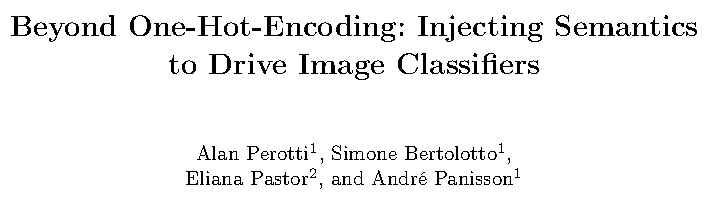
\includegraphics[width=.8\linewidth]{figures/02/paper_title.pdf}
  \end{figure}
  \begin{figure}
    \centering
    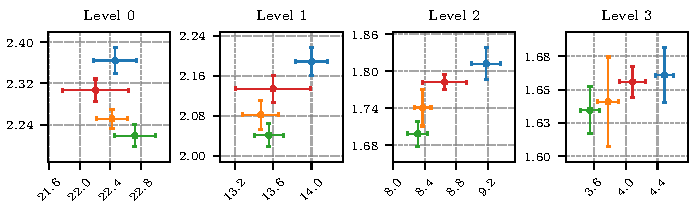
\includegraphics[width=.8\linewidth]{figures/02/paper_errors.pdf}
  \end{figure}
  \begin{figure}
    \centering
    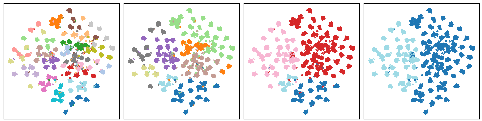
\includegraphics[width=.8\linewidth]{figures/02/paper_features.pdf}
  \end{figure}

  \note{\scriptsize{Questa tecnica per sfruttare le reazioni tra classi usando un
    esplicita gerarchia, è stata già descritta in alcune pubblicazioni.
    Una di queste è un articolo che sarà presentato a xAI 2023.}}
  \note[item]{Abbiamo applicato una simile tecnica per produrre un embedding
    gerarchico e confrontato le performance con quelle ottenute da modelli
    che sfruttano e non la gerachica tra le classi.}
  \note[item]{Per performance intendiamo la quatità di errori, asse orizzontale, e
    la qualità degli errori, asse verticale, a diversi livelli della gerarchica.
    Questi plots saranno ripresi in seguito.}
  \note[item]{Abbiamo inoltre studiato la disposizione spaziale dei features
    vectors, ovvero come sono organizzati nello spazio i vettori del penultimo
    livello del modello associati alle varie immaginni}
  \note[item]{Proiettarli nel piano dà un'indicazione su quali immagini il
    modello pensa siano simili. Ciò che ci attendiamo è la comparsa di cluster
    relativi alle varie classi.}
  \note[item]{Abbiamo usato delle metriche di clustering per quantificare il
    raggruppamento dei features vectors e capire quali modelli producevano una
    rappresentazione interna più strutturata.}
  \note[item]{Un limite di tale approccio è la necessità di avere o poter
    costruire una gerarchica tra le classi. Uno degli approcci presentati supera
    tale limite ricavando gli encoding dai word embeddings delle classi. Ma ciò
    introduce un altri problemi, non tutte le parole hanno un'embedding e una
    parola può avere diversi un significati.}
  \note[item]{Da qui l'idea dei descriptions encodings.}
\end{frame}
